\section{Problema de planificación de producción tipo taller (JSP)}

Dentro de los problemas de planificación, el JSP modela un taller en el que hay $m$ máquinas, cada una de las cuales puede hacer varios tipos 
de procedimientos pero solo puede hacer uno de ellos a la vez. 
%
Se requiere completar $n$ trabajos, cada uno de los cuales está compuesto por $m$ operaciones, una por cada máquina en el taller, y que deben 
procesarse en un orden específico y por un tiempo específico en cada una de ellas. 

Por ejemplo una panadería puede modelarse del siguiente modo; las herramientas como batidora, rodillo, horno, etc. pueden representarse como las
$m$ máquinas que se utilizan en un orden determinado para hacer $n$ distintos tipos de pan, los cuales pueden representarse como los trabajos 
a completar.

Las secuencias y tiempos de procesamiento para cada trabajo deben de especificarse para definir el problema. 
%
Habitualmente se presentan en una tabla de $n$ renglones por $m$ columnas esto se conoce como una instancia del JSP. 
%
Para cada renglón, las columnas contienen, de forma ordenada, la máquina en que debe procesarse el trabajo en cada paso y el tiempo 
que toma procesarlo. 
%
Por ejemplo en la tabla~\ref{tab:inst} se presenta una instancia del JSP con 3 máquinas y 2 trabajos. 
%
En esta instancia el trabajo 1 debe procesarse primero en la máquina 0 por 75 unidades de tiempo, luego en la máquina 2 por 54 unidades de tiempo y 
por último en la máquina 1 por 59 unidades de tiempo.

El problema a resolver consiste en hallar una planificación que sea óptima en algún sentido y respete los requisitos impuestos (orden y no concurrencia de diversas
operaciones).
%
Así, una planificación consiste en asignar tiempos de inicio y fin a cada operación respetando el orden requerido para cada trabajo. 
%
Existen varias formas de determinar si una planificación es óptima como se explicará más adelante pero la más usada es el tiempo que toma terminar la última operación.
%
A este timpo se le conoce como makespan. 
%
Sin pérdida de generalidad nos restringirnos al caso en el que el tiempo requerido para procesar cada operación es un entero positivo.

%Indicar que surgen dos tipos de dependencias, una en las propias máquinas (no puedes empezar antes que tu predecesora), y otra entre trabajos (no puedes empezar
%hasta que acabe de predecesor del trabajo).
%Es difícil definir el concepto de ruta crítica, sin decir que se hace uso de soluciones semi-activas, entonces creo que es importante definir aquí ese concepto
%Hay que ser más formal al definir la ruta crítica, algo así como secuencia de operaciones tales que cada una tiene dependencia con la anterior, en la que la primera 
%empieza en el tiempo 0 de planificación y la última termina en el tiempo makespan, y que cumple además que, cada operación empieza justo al terminar la operación
%anterior de la secuencia
Otro concepto que es de gran utilidad en los métodos que se presentarán en las siguientes secciones es la secuencia de trabajos que toma el mayor tiempo en 
completarse conocida como \textbf{ruta crítica}. 
%
Esta ruta crítica se compone a su vez de una serie de bloques críticos que consisten en las secuencias de operaciones de la ruta crítica que se ejecutan de forma 
adyacente en la misma máquina. 
%
Es importante mencionar que una planificación siempre tiene al menos una ruta crítica pero puede tener más de una a la vez.

Es muy usual que una planifacación se visualice mediante un diagrama de gantt. 
%
El siguiente ejemplo sirve para mostrar los conceptos antes presentados en un caso práctico y simple.

\subsection*{Ejemplo}
Se muestra un ejemplo de una instancia con 3 máquinas y 2 trabajos.
\begin{table}[H]
\centering
\begin{tabular}{@{}llll@{}}
Trabajo & \multicolumn{3}{l}{\begin{tabular}[c]{@{}l@{}}Secuencia de procesamiento \\ (máquina, tiempo)\end{tabular}} \\ \midrule
0       & 0, 75                              & 2, 54                               & 1, 59                             \\ \midrule
1       & 0, 47                              & 2, 72                              & 1, 45   \\\hline                         
\end{tabular}
\caption{Instancia simple con 3 maquinas y 2 trabajos}
\label{tab:inst}
\end{table}

La siguiente es una posible planificación para la instancia de ejemplo, visualizada mediante un diagrama de gantt. En negro se marcan los trabajos que conforman la ruta crítica. 
\begin{figure}[H]
\centering
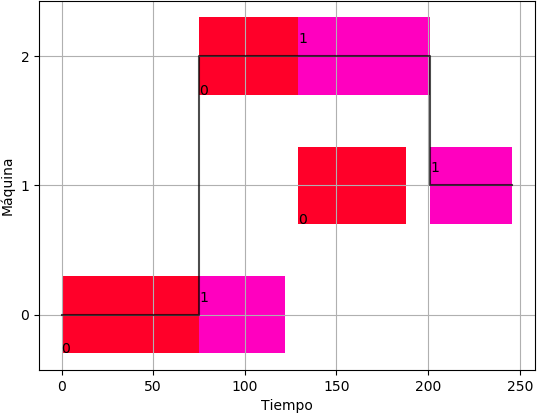
\includegraphics[scale=.7]{Imagenes/planejemplorc.png}
\caption{Diagrama de gantt de una planificación posible}
\label{fig:gantt}
\end{figure}

Si bien es conveniente visualizar una planificación mediante un diagrama de gantt como el mostrado anteriormente, resulta ventajoso representar computacionalmente 
estas planifaciones de otras formas. 
%
La representación de soluciones a un problema resulta ser una elección sumamente importante al momento de desarrollar, implementar y analizar los algoritmos que se 
propongan para resolver el problema~\cite{rothlauf2002representations}. 
%
En la siguiente sección se detallan dos formas de representación de especial importancia.

\subsection{Representación de planificaciones}
De manera general las representaciones para el JSP se pueden clasificar en\cite{Cheng1996}:
\begin{itemize}
    \item \textbf{Representación directa}: Se almacena el orden de los trabajos en cada máquina o sus tiempos de inicio y final.
    \item \textbf{Representación indirecta}: Se almacena información con la que se puede construir una planificación mediante un proceso de decodificación.
\end{itemize}

En este trabajo se utilizaron dos: el grafo disyuntivo (representación directa) y las reglas de prioridad (representación indirecta).
\subsubsection*{Modelo de grafo disyuntivo} 
En este modelo las planificaciones se representan con un grafo dirigido $G=(V,A,E)$ en el que $V$ es un conjunto de nodos que representa las operaciones, las aristas $A$ representan la secuencia que deben seguir las operaciones dentro de un mismo trabajo y $E$ es otro conjunto de aristas que indica el orden de procesamiento en cada una de las máquinas. Es importante mencionar que con este modelo podemos representar planificaciones no factibles, esto se da cuando el grafo $G$ contiene un ciclo.


Formalmente en una instancia del JSP se representa cada operación como un nodo, se agregan dos nodos de control que sirven como el nodo inicial (del que dependen todos los trabajos) y final (que depende de todos los trabajos), las restricciones de precedencia dentro de cada trabajo se representan como aristas dirigidas fijas llamadas aristas conjuntivas y las operaciones que deben procesarse en una misma máquina se unen mediante aristas llamadas disyuntivas, una solución factible o planificación se obtiene al elegir la dirección para cada arista disyuntiva de modo que no se generen ciclos.   
%El problema de hallar una planificación para cada una de las $m$ operaciones de los $n$ trabajos en las $m$ máquinas se reduce a elegir una permutación de los $n$ trabajos en cada máquina por lo que el número de posibles soluciones es $O(n!^m)$.

% poner las representaciones
\begin{figure}
    \centering
    \begin{subfigure}{.8\textwidth}
        \centering
        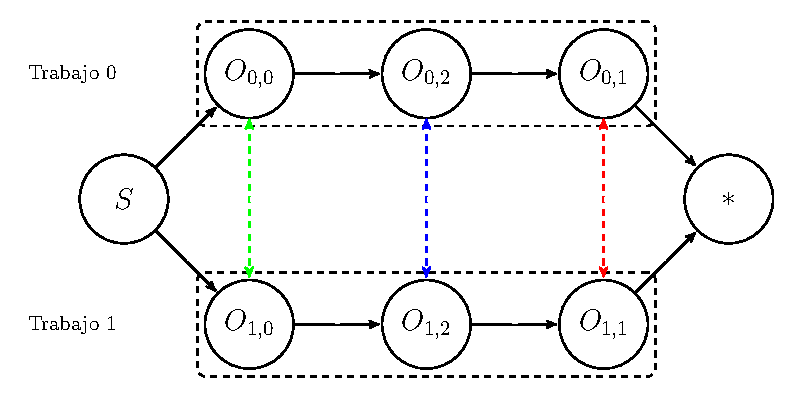
\includegraphics[width=.8\linewidth]{Imagenes/disyuntive.pdf}
        \caption{Representación de una instancia, los colores distinguen entre las tres máquinas.}
    \end{subfigure}
    \begin{subfigure}{.8\textwidth}
        \centering
        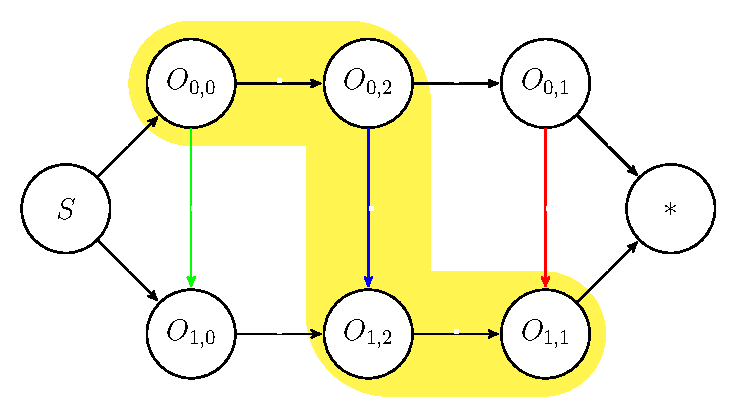
\includegraphics[width=.8\linewidth]{Imagenes/plandisyuntive.pdf}
        \caption{Planificación obtenida al fijar las aristas disyuntivas como en \ref{fig:gantt}. La ruta critica se resalta en amarillo}
    \end{subfigure}
\caption{Modelo de grafo disyuntivo para la instancia de ejemplo \ref{tab:inst}}
\end{figure}

\subsubsection*{Reglas de prioridad}
En esta representación una planificación se construye al aplicar un proceso de simulación en el que para cada maquina se construye una cola con las operaciones cuyas dependencias ya han sido procesadas. Inicialmente se tienen en las colas solo las operaciones iniciales de cada trabajo. Una vez que se tiene esto se utiliza una regla de prioridad para elegir qué operación debe planificarse en qué máquina. Se actualizan las colas para las máquinas que lo requieran y se continua con este proceso hasta completar la planificación (vaciar las colas).

Existen muchas reglas de prioridad que toman en cuenta cosas como la duración de la operación, la cantidad de operaciones restantes, la duración del trabajo al que pertenece una operación, entre muchas otras. La calidad de la planificación construida depende de la regla de prioridad que se utilice y de la estructura de la instancia en sí.


\subsection{Tipos de planificaciones}
Independientemente de cómo se representen o como se construyan las planificaciones pueden clasificarse en varios conjuntos. Dentro de el conjunto de planificaciones factibles se pueden distinguir dos subconjuntos de interés para el presente trabajo: el conjunto de las planificaciones óptimas que está conformado por las planificaciones con el menor makespan posible y el conjunto de las planificaciones activas. 
Estas últimas se definen como las planificaciones en las que no es posible disminuir el tiempo de inicio de ninguna operación sin aumentar el tiempo de inicio de otra. Es conocido que las planificaciones óptimas representan un subconjunto de las activas\cite{Ponsich2013}.

% imagen 

\begin{figure}[H]
    \centering
    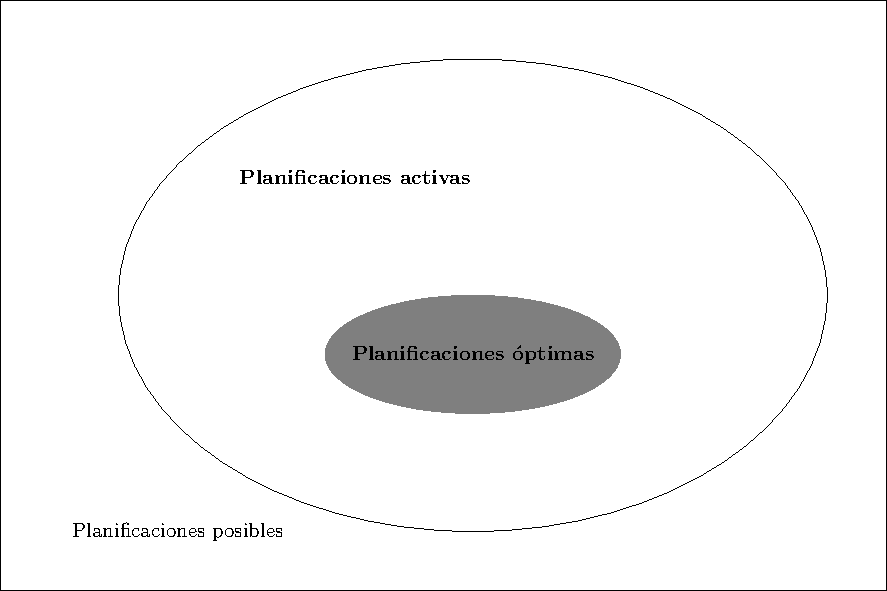
\includegraphics[scale=.8]{Imagenes/solspace.pdf}
    \caption{Subconjuntos de planificaciones}
\end{figure}

Estas clasificaciones resultan interesantes porque existen algoritmos para generar tipos de planificaciones de modo que podamos centrarnos en solo un subconjunto del espacio de búsqueda.
